\documentclass[margin=0mm, innermargin=3cm, blockverticalspace=15mm, colspace=15mm, subcolspace=8mm, a0paper, titleinnsersep = 0pt]{tikzposter}
\usepackage{graphicx} 
\usepackage[utf8]{inputenc}
\usepackage{xcolor}
\usepackage{tikz}
\usetikzlibrary{shapes.geometric, arrows.meta}
\usepackage[ngerman]{babel}
\usepackage{multicol}
\usepackage{wrapfig}
\tikzposterlatexaffectionproofoff %Tikzposter Wasserzeichen ausblenden
\usetikzlibrary{babel}
\setlength{\columnsep}{2cm}

%Abbildungsreferenzen Deutsch
\addto\captionsngerman{
  \renewcommand{\figurename}{Abb.}
  \renewcommand{\tablename}{Tab.}
}

%Titel
\title{\parbox{0.6\linewidth}{\centering Robustness of machine learning against Batch effects in RNA-seq data}}

%Farbpalette in TH-Farbe von Originalvorlage
\definecolorpalette{thpalette} {
    \definecolor{thblue}{RGB}{0,91,153}
}

%Hintergrund: Rahmen etc.
\definebackgroundstyle{frame}{
    %Aussenrahmen
    \draw[inner sep=0pt, line width=30pt, color=thblue, fill=white]
    (-40,-57) rectangle (40, 57);
    %Linien box Praxisphase von x,y
    \draw[line width=15pt, color=thblue] (-40,45) -- (40,45);
    \draw[line width=15pt, color=thblue] (-40,39) -- (40,39);
    %Linien box Durchgefuehrt bei: Betrieb, Ort
    %\draw[line width=15pt, color=thblue] (-40,-45) -- (40,-45);
    \draw[line width=15pt, color=thblue] (-40,-51) -- (40,-51);
}

%Titel Style
\definetitlestyle{thtitle}{
    width=\paperwidth, roundedcorners=0, linewidth=0pt, innersep=1.5cm,
    titletotopverticalspace=5cm, titletoblockverticalspace=6cm,
    titlegraphictotitledistance=1pt, titletextscale=1
}{}

%Block Style
\defineblockstyle{thblocks}{
titlewidthscale=0.9, bodywidthscale=1,titleleft,
titleoffsetx=0pt, titleoffsety=3mm, bodyoffsetx=0mm, bodyoffsety=19mm,
bodyverticalshift=18mm, roundedcorners=5, linewidth=2pt,
titleinnersep=6mm, bodyinnersep=1cm
}{
\draw[color=thblue, fill=blockbodybgcolor] (blockbody.south west)
rectangle (blockbody.north east);
\ifBlockHasTitle
\draw[color=thblue, fill=thblue] (blocktitle.south west)
rectangle (blocktitle.north east);
\fi
}

%TH layout definieren
\definelayouttheme{th}{
    \usebackgroundstyle{frame}
    \usecolorpalette{thpalette}
    \usetitlestyle{thtitle}
    \useblockstyle{thblocks}
}

\usetheme{th} 
\begin{document}

%Logos einfuegen
\node (thlogo) at (32, 51) {
\includegraphics[width=10cm]{bingen.pdf}};
\node (betrieb) at (-32, 51) {
\includegraphics[width=10cm]{mainz.png}};

%Praxisphase von Vorname Name
\node [above right,
    outer sep=0pt,
    fill opacity=0,
    line width=0mm,
    text opacity=1,
    minimum width=80cm,
    minimum height=6cm,
    align=center,font=\Huge,
    draw=none,fill=white] at ([shift={(0.5*\pgflinewidth,0.5*\pgflinewidth)}]-40,39) {Practical phase of Laszlo Lang\\Supervised by Dr. Maximilian Sprang – The Mayer Lab Mainz};

%Durchgefuehrt bei Firma, Ort
%\node [above right,
%    outer sep=0pt,
%    fill opacity=0,
%    line width=0mm,
%    text opacity=1,
%    minimum width=80cm,
%    minimum height=6cm,
%    align=center,font=\Huge,
%    draw=none,fill=white] at ([shift={(0.5*\pgflinewidth,0.5*\pgflinewidth)}]-40,-51) {Durchgeführt bei: %Betrieb, Ort};

%Studiengang Angewandte Bioinformatik
\node [above right,
    outer sep=0pt,
    fill opacity=0,
    line width=0mm,
    text opacity=1,
    minimum width=80cm,
    minimum height=6cm,
    align=center,font=\Huge,
    draw=none,fill=white] at ([shift={(0.5*\pgflinewidth,0.5*\pgflinewidth)}]-40,-57) {Bachelor's Degree Program „Angewandte Bioinformatik“};

\maketitle[]


\begin{columns}
\column{}
%Bloecke mit Inhalt
\block{Introduction}{
	\fontsize{26}{25}\selectfont
	RNA sequencing (RNA-seq) enables the systematic study of gene expression and provides insights into biological processes at the molecular level. However, RNA-seq data are often affected by batch effects. 
	These arise from systematic technical variation, for example, due to sequencing runs, sample preparation, or laboratory conditions. Such variation can obscure true biological signals and complicate downstream analyses. Machine learning (ML) methods are powerful tools for detecting complex patterns in high-dimensional data. Yet, in the context of RNA-seq, it remains unclear whether ML models capture genuine biological variation or adapt to technical artifacts.\\
In this project, we investigate the robustness of selected ML methods against batch effects in RNA-seq data. Classical differential expression analysis is compared with ML-based approaches, and the resulting gene lists are interpreted in biological context using over-representation analysis (ORA) and correlation analysis. This allows us to highlight differences between methods and assess which biological pathways remain consistently detectable despite batch effects.
} 
\end{columns}
\begin{columns}
\column{}
\block{Workflow \& Methodology}{
\fontsize{26}{25}\selectfont
	\begin{tikzpicture}[node distance=2cm]
    		\definecolor{thgreen}{RGB}{166,204,115}
    		\definecolor{mzblue}{RGB}{128,161,202}
		\tikzstyle{io} = [trapezium, trapezium left angle=70, trapezium right angle=110, minimum width=3cm, minimum height=1cm, text centered, draw=black, fill=mzblue!100]
	\tikzstyle{process} = [rectangle, minimum width=3cm, minimum height=1cm, text centered, draw=black, fill=thgreen!100]
		\tikzstyle{arrow} = [-{Stealth[length=5mm]}]
		
		\node (input) [io, align=left] {Python: Data Input};
		\node (preparation) [process, below of=input, yshift=-1.5cm, align=left] {Data Preparation};
		\node (normalization) [process, right of=preparation, xshift=7.5cm, align=left] {Normalization};
		\node (logreg) [process, right of=normalization, xshift=7.5cm, yshift=2.5cm, align=left] {Logistic Regression};
		\node (randforest) [process, right of=normalization, xshift=7.5cm, yshift=-2.5cm, align=left] {Random Forest};
		\node (ml_features_output) [io, right of=logreg, yshift=-2.5cm, xshift=7.5cm, align=left] {ML-Features};
		\node (counts_output) [io, below of=preparation, yshift=-1.5cm] {Counts Output};
		
		\node (counts_input) [io, right of=ml_features_output, xshift=9cm] {R: Counts Input};
		\node (DGE) [process, right of=counts_input, align=left, yshift=2.5cm, xshift=10cm] {Differential Expression};
		\node (BatchCor) [process, right of=counts_input, align=left, yshift=-2.5cm, xshift=10cm] {Batch Correction};
		\node (ora) [process, right of=DGE, yshift=-2.5cm, xshift=10cm, align=left] {Downstream Analysis};\\
		%- Over-Representation Analysis\\
		%- Correlation Analysis};
		\node (ml_features_input) [io, above of=ora, xshift=5cm, yshift=1cm] {ML-Features};
		%\node (results) [io, right of=ora, align=left, xshift=15.5cm] {Results\\
		%- Comparison of ML vs. classical approaches\\
		%- Consistently enriched pathways across methds};
		
		\draw [-{Stealth[length=5mm]}] (input) -- (preparation);
		\draw [-{Stealth[length=5mm]}] (preparation) -- (normalization);
		\draw [-{Stealth[length=5mm]}] (normalization) |- (logreg);
		\draw [-{Stealth[length=5mm]}] (normalization) |- (randforest);
		\draw [-{Stealth[length=5mm]}] (logreg) -| (ml_features_output);
		\draw [-{Stealth[length=5mm]}] (randforest) -| (ml_features_output);
		\draw [-{Stealth[length=5mm]}] (preparation) -- (counts_output);
		
		%\draw [-{Stealth[length=5mm]}] (counts_output) -| (counts_input);
		%\draw [-{Stealth[length=5mm]}] (ml_features_input) -- (ml_features_output);
		
		\draw [-{Stealth[length=5mm]}] (counts_input) |- (DGE);
		\draw [-{Stealth[length=5mm]}] (counts_input) |- (BatchCor);
		\draw [-{Stealth[length=5mm]}] (DGE) -| (ora);
		\draw [-{Stealth[length=5mm]}] (BatchCor) -| (ora);
		\draw [-{Stealth[length=5mm]}] (ml_features_input) -- (ora);
		%\draw [-{Stealth[length=5mm]}] (ora) -- (results);
	\end{tikzpicture}
\linebreak\linebreak
An HCC RNA-seq dataset was analyzed with four feature selection strategies: classical Differential Gene Expression analysis (DGE), batch-corrected DGE (BatchCor), Logistic Regression (LogReg) and Random Forest Classification (RandForest). Each method was used to identify the top 1000 features, which were then used for over-representation analysis (ORA) to extract the top 100 pathways.\\Overlaps between feature lists and pathway lists were visualized with Venn diagrams. To evaluate the stability of selected signatures under batch effects, two correlation analyses were performed.\\One compares each dataset with the feature lists identified by a method with and without the outlier. The other compares each dataset with method-specific consistent features (intersection, $\cap$, found in both conditions) versus variable features (symmetric difference, $\Delta$, found only in one condition), focusing on features uniquely detected by the respective method.

}
\end{columns}

\begin{columns}
\column{}
\block{Downstream Analysis Results}{
\fontsize{26}{25}\selectfont
\begin{minipage}{0.65\textwidth}
\textbf{Feature-Level Overlaps (Top 1000 Features):}
\begin{itemize}
\item \textbf{With Outlier}: 61 features shared across all methods; most are method-specific (RandForest: 842; LogReg: 737; DGE: 45; BatchCor: 34).
\item \textbf{Without Outlier}: Common overlap drops to 42; DGE/BatchCor lose many unique features (45 $\rightarrow$ 24; 34 $\rightarrow$ 23).
\item Random Forest and Logistic Regression remain similar (873 and 738 unique), but largely method-exclusive.
\item Only 18 features are shared in both conditions $\Rightarrow$ even the common core is unstable.
\end{itemize}
\vspace{0.25em} \textbf{Interpretation:} ML-based methods yield stable counts but mostly method-specific feature sets with limited overlap to each other and to classical approaches. In contrast, DGE and BatchCor show the largest overlap, consistent with their shared methodology. Overall, classical methods converge on more similar signatures, whereas ML approaches produce distinct yet internally stable sets, raising concerns about the robustness of feature selection.
\end{minipage}
\hfill 
\begin{minipage}{20cm}
        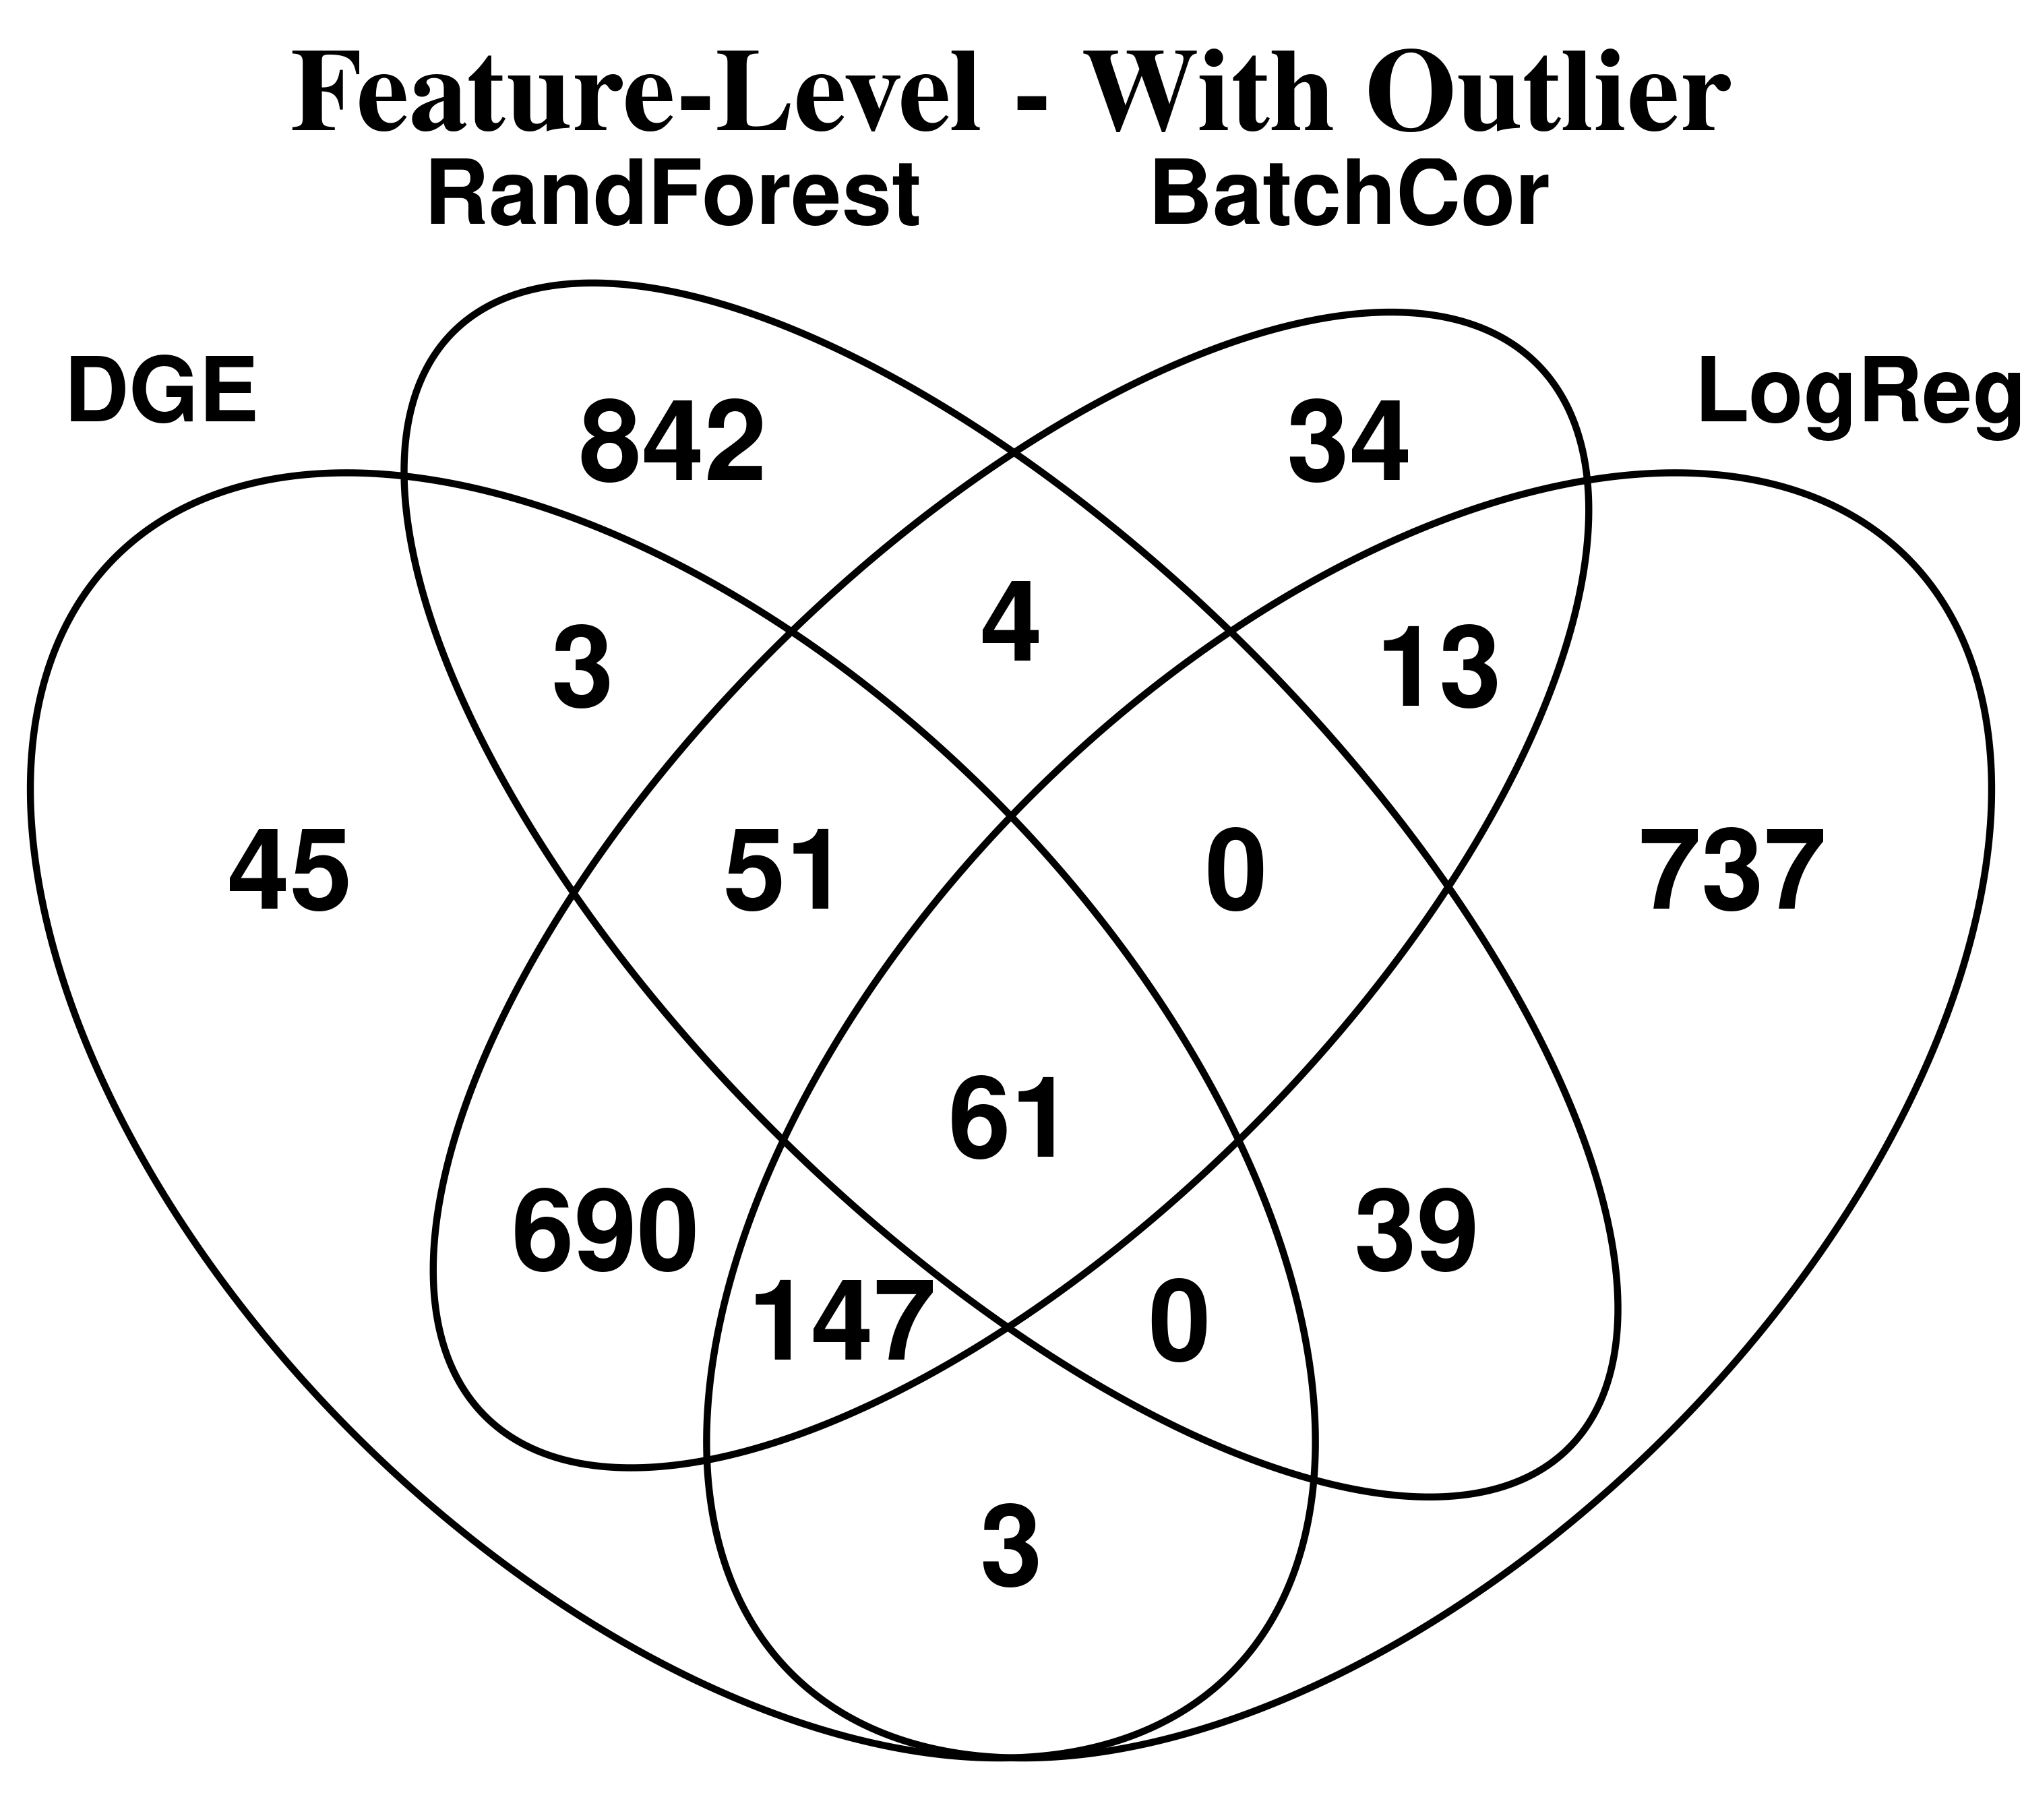
\includegraphics[width=9cm]{features_with_outlier.png}
		\hfill
        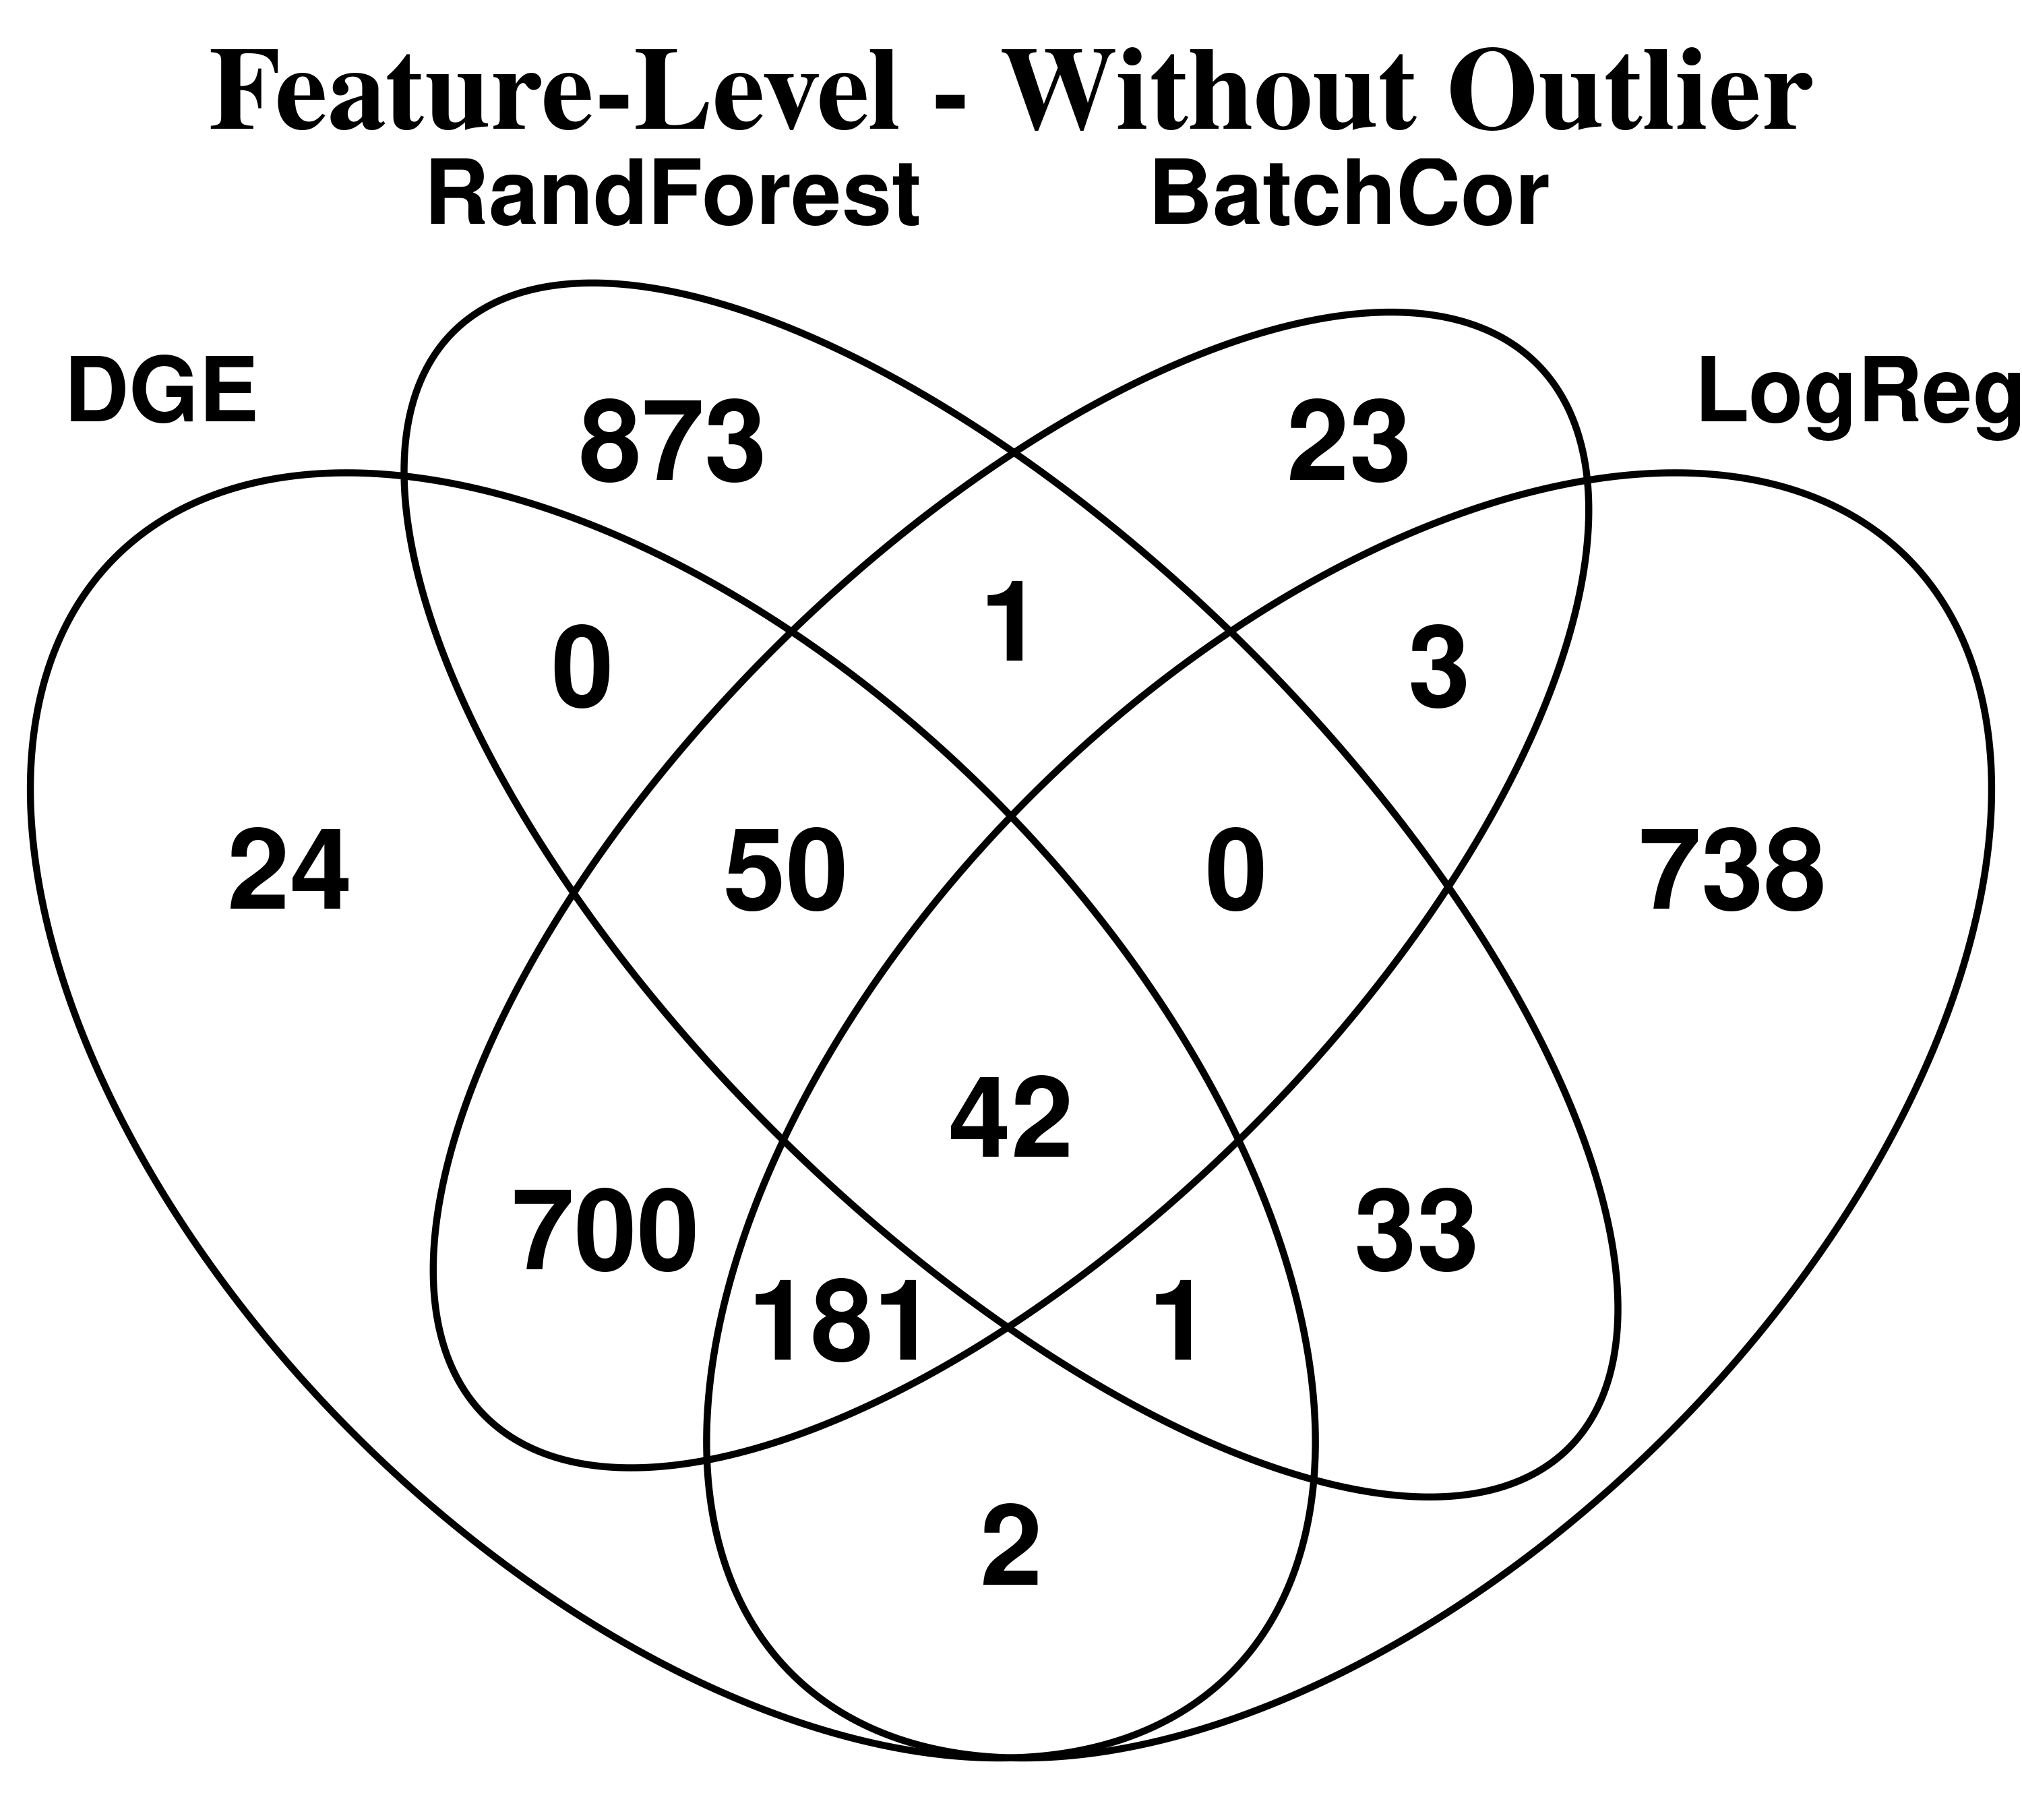
\includegraphics[width=9cm]{features_without_outlier.png}
        
\end{minipage}

\vspace{0.75cm}
\begin{minipage}{0.65\textwidth}
\textbf{Pathway-Level Overlaps (Top 100 Pathways):}
\begin{itemize}
\item \textbf{With Outlier}: 42 pathways shared across all methods.
\item \textbf{Without Outlier}: Overlap rises slightly to 45.
\item Only 29 pathways are identical in both conditions $\Rightarrow$ shared core is limited.
\item Unique pathways: RandForest 37 $\rightarrow$ 40; LogReg 26 $\rightarrow$ 24; DGE 2 $\rightarrow$ 2; BatchCor 2 $\rightarrow$ 0.
\end{itemize}
\vspace{0.25em} \textbf{Interpretation:} A moderate pathway core is consistently recovered, but many remain method-specific. DGE and BatchCor show strong overlap, whereas ML methods yield more distinct results. Thus, enrichment outcomes are partly robust but also shaped by method-related artifacts, which limits the reliability of unique findings.
%\end{itemize}
\end{minipage}
\hfill 
\begin{minipage}{20cm}
    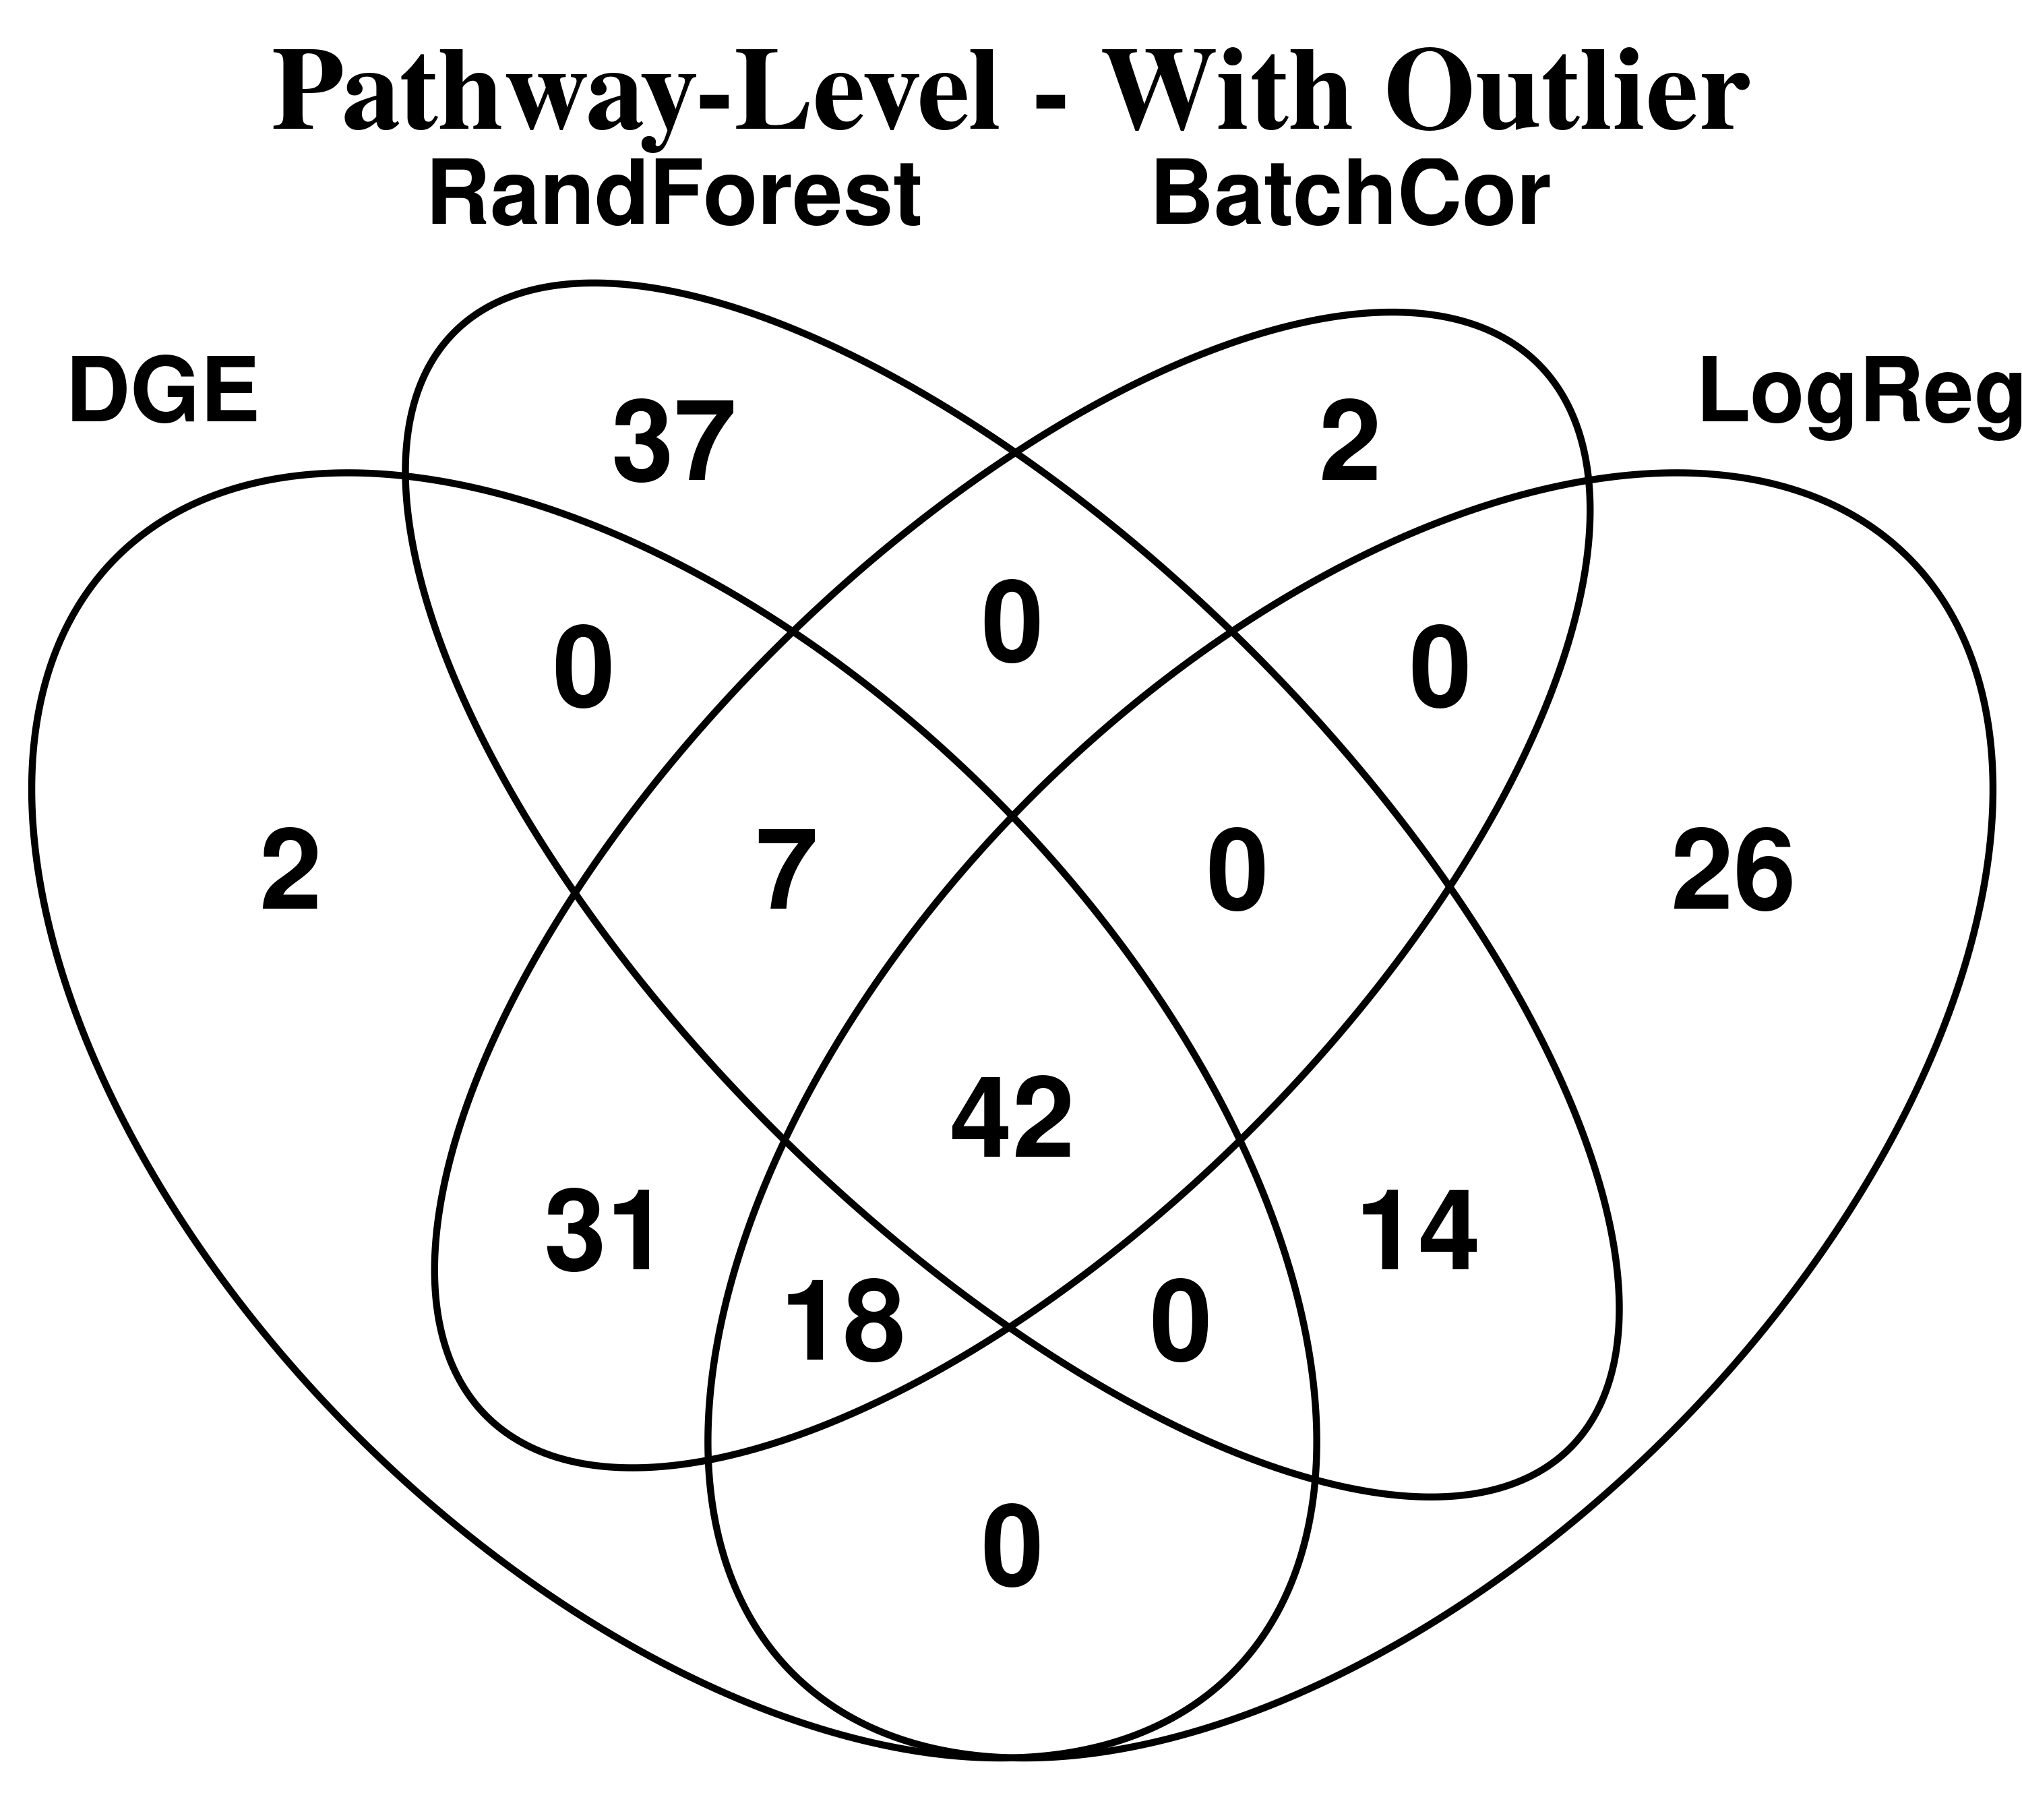
\includegraphics[width=9cm]{pathways_with_outlier.png}
	\hfill
	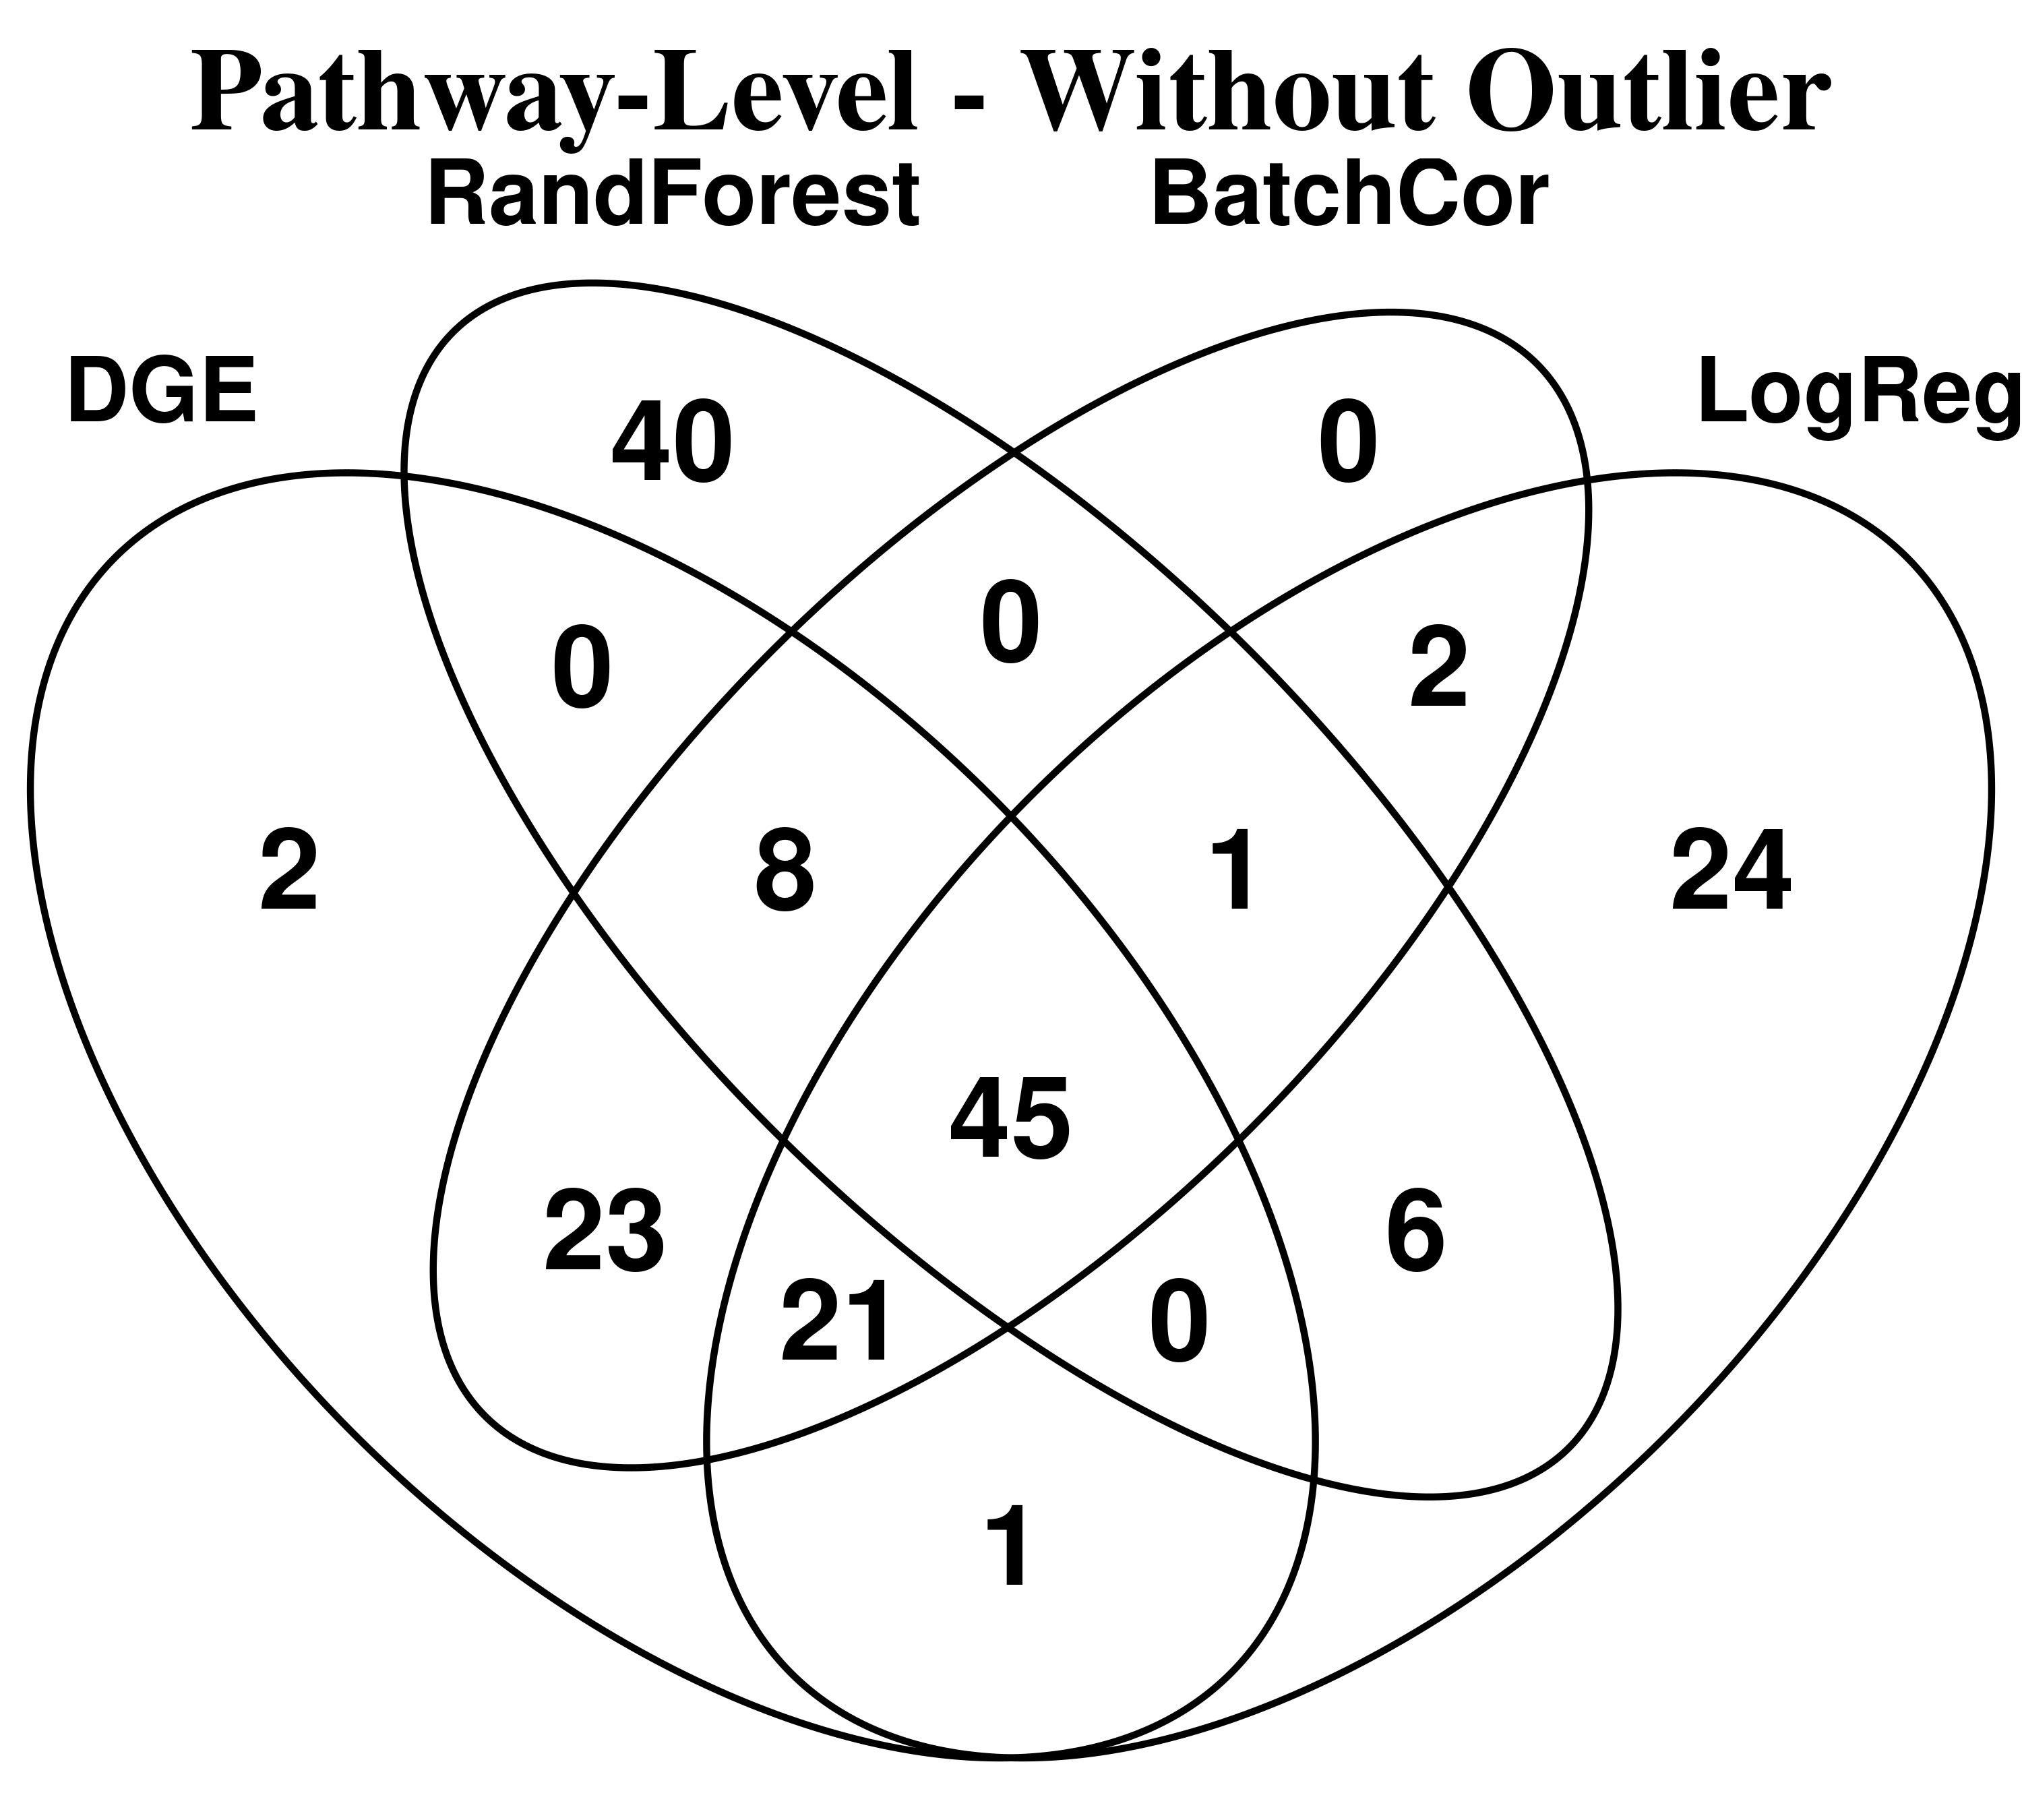
\includegraphics[width=9cm]{pathways_without_outlier.png}   
\end{minipage}
\vspace{0.5cm}
\begin{minipage}{0.6\textwidth}
\textbf{Correlation Analysis:}\\[0.25em]
\textbf{Method-Derived Feature Sets:}\\
Features identified by each method showed very high correlations across most datasets, confirming stable expression patterns.\\The outlier dataset GSE144269 was a clear exception, where correlations dropped significantly, confirming its disruptive effect.\\Correlation levels varied slightly between methods, reflecting differences in feature selection strategies.\\[0.5em]
\textbf{Method-Specific Feature Sets:} %Consistent features are defined as the intersection ($\cap$), and variable features as the symmetric difference ($\Delta$), of features identified only by the respective method with and without the outlier dataset.
\begin{itemize}
\item \textbf{DGE:} Produces many more variable than consistent features; the consistent set shows markedly lower correlations, in some cases approaching zero or negative values.
\item \textbf{Batch Correction:} Nearly perfect correlations ($\sim$ 0.99 - 1.0), suggesting effective batch adjustment and robustness.
\item \textbf{Random Forest:} Very high correlations for both consistent and variable features ($\sim$ 0.97 - 0.99), indicating strong stability.
\item \textbf{Logistic Regression:} Solid correlations ($\sim$ 0.84 - 0.96), somewhat lower but still robust.
\end{itemize}
\vspace{0.25em} \textbf{Interpretation:}
Correlation analysis suggests that features consistently detected across methods represent robust biological signals. Random Forest and Batch Correction appear to produce the most stable signatures, while DGE seems sensitive to dataset variability and outliers.
\end{minipage}
\hfill
\begin{minipage}{25cm}
	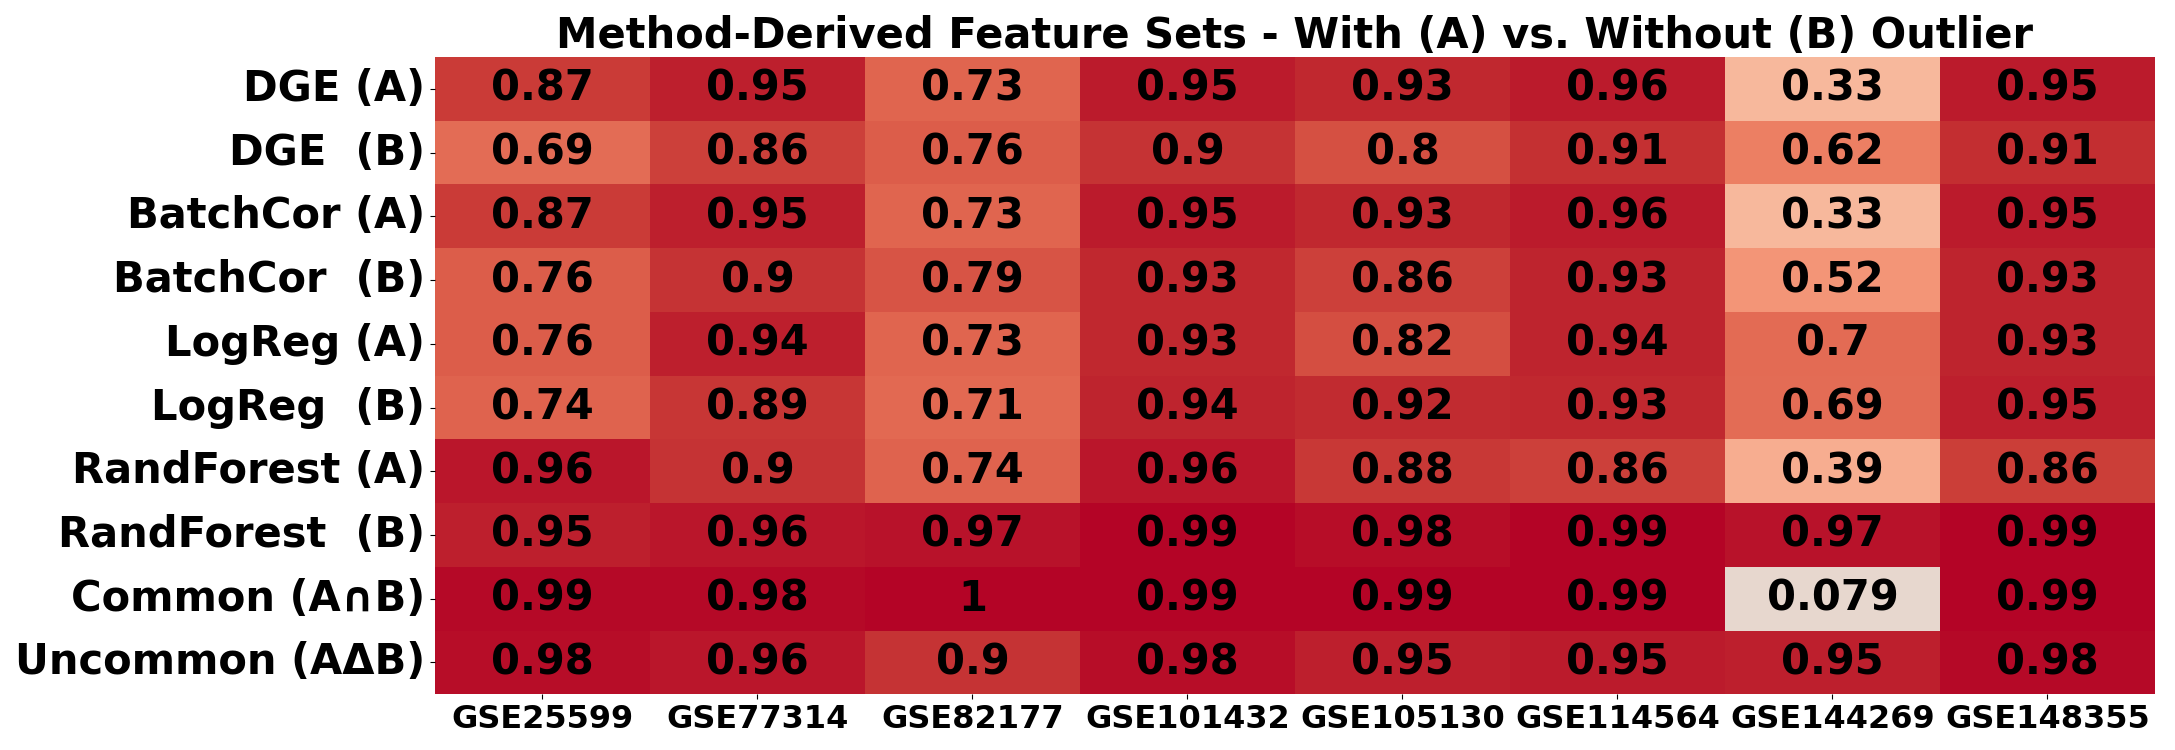
\includegraphics[width=25cm]{correlation_method.png}
	\hfill
    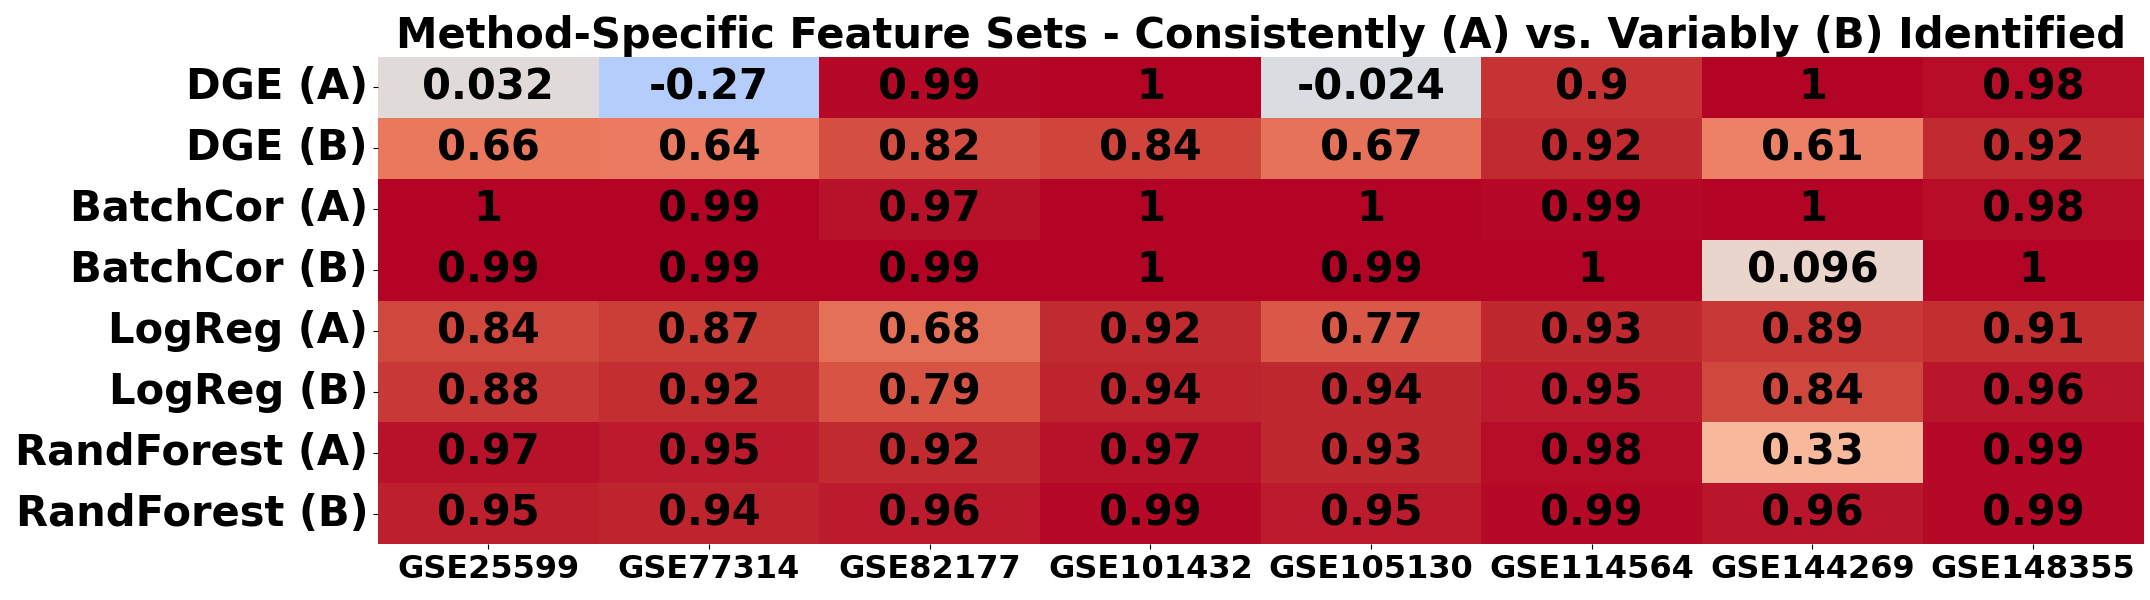
\includegraphics[width=25cm]{correlation_unique.png}
\end{minipage}
}
\end{columns}
\begin{columns}
\column{}
\block{Abstract / Conclusion}{
\fontsize{26}{25}\selectfont
This work evaluates the robustness of machine learning versus classical approaches for RNA-seq feature selection under batch effects.
\begin{itemize}
\item \textbf{Feature-Level:} Overlaps between methods are limited (61 features with the outlier, 42 without; 18 identical), with most features being method-specific. DGE and BatchCor lose many unique features once the outlier is removed, yet they still show the largest mutual overlap overall. In contrast, RandForest and LogReg remain relatively stable but largely distinct from the classical approaches.
\item \textbf{Pathway-Level:} A moderate overlap is observed (42 pathways with the outlier, 45 without; 29 identical). DGE and BatchCor show the strongest agreement, while ML approaches contribute many method-exclusive pathways, questioning the reliability of unique results.
\item \textbf{Correlation:} Consistent features show stable expression patterns across datasets, with the outlier being the main exception. Among methods, Random Forest and BatchCor yield the most stable correlation profiles, whereas DGE appears more sensitive to dataset variation.
\end{itemize}
\textbf{Limitations:} The analysis is based on a single dataset (HCC) with strong expression signals, and the true ground truth is unknown.\\
\textbf{Improvment:} Validation on additional datasets (e.g., glioblastoma or diseases with weaker DEG signals) and on simulated data with defined ground truth would help confirm these findings.\\[0.5em]
\textbf{Final assessment:} The results suggest that machine learning methods such as Random Forest may be less affected by batch variation, while classical methods converge more strongly on shared results.\\Both strategies reveal a partly stable biological core at the pathway level, but substantial method-specific differences remain.\\Broader validation is needed to assess whether ML models capture robust biology or adapt to technical artifacts.
}

\end{columns}
%\begin{multicols}{2}
%\columnbreak
%\end{multicols}
%\textbf{Gene-level Feature Overlap}\\
%Test Tes
\end{document}